\documentclass[11pt]{beamer}
\usetheme{Szeged}
\usepackage[utf8]{inputenc}
\usepackage[french]{babel}
\usepackage[T1]{fontenc}
\usepackage{amsmath}
\usepackage{amsfonts}
\usepackage{amssymb}
\usepackage{listings} 
\author{\texorpdfstring{Samy Aittahar\newline\url{saittahar@ulg.ac.be}}{Samy Aittahar}}
\title{Prolog : Preliminaries}

%\setbeamercovered{transparent} 
%\setbeamertemplate{navigation symbols}{} 
%\logo{University of Liège} 
\institute{University of Liège} 
\date{\today} 
%\subject{} 
\begin{document}
\lstset{language=Prolog}  
\begin{frame}
\titlepage
\end{frame}


\begin{frame}{Me in a nutshell}

	\begin{itemize}
	
		\item PhD Student in computer science ;
		\item Main research : Transfer learning for deep reinforcement learning ;
		\item \url{http://www.montefiore.ulg.ac.be/~saittahar/} 
	
	\end{itemize}

\end{frame}

\begin{frame}{Practical informations}
\begin{itemize}
	\item Format : Project presentations, with homeworks in a "two-weekly" basis.
	\item Mail subject pattern for homeworks : \emph{Lastname\_ Firstname} Homework $N$ \;,
	\item When attaching a bonus step to the homework, append [Bonus] to the subject.
\end{itemize}
\end{frame}

\begin{frame}{Facts and search trees}

\begin{itemize}
	\item A fact is a logical statement, represented by a first-order logical predicate ;
	\item Depth-first searching algorithm through a given database of facts and predicates;
	\begin{itemize}
	   \item Goes backward when either unification fails or succeed ;
	\end{itemize}
	\item Pro : enumerates all possible solutions ;
	\item $/!\backslash $ Even if logically equivalent, order of facts often matters for computational efficiency !
	\end{itemize}

\end{frame}

\begin{frame}[fragile]{Example 1 - Facts}

\begin{lstlisting}
ancestor(X,X).
ancestor(X,Y) :- parent(X,Z), ancestor(Z,Y).
parent(amy,bob).
\end{lstlisting}

\end{frame}

\begin{frame}[fragile]{Tree Search (Example 1)}

	\begin{lstlisting}[xleftmargin=.27\textwidth]
ancestor(X,bob).
\end{lstlisting}

\begin{center}

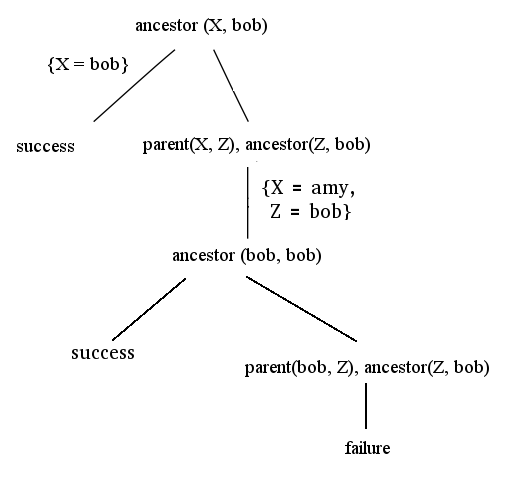
\includegraphics[scale=0.5]{resolution_1.png}
\end{center}

\end{frame}

\begin{frame}[fragile]{Example 2 - Lists}

	Member of a list :
	\begin{lstlisting}
member(X,[X|LX].
member(X,[Y|LX]) :- member(X,LX).
\end{lstlisting}

\end{frame}

\begin{frame}[fragile]{Tree Search [Example 2]}

\begin{lstlisting}[xleftmargin=.17\textwidth]
member(X,[a,b,c]).
\end{lstlisting}

\begin{center}

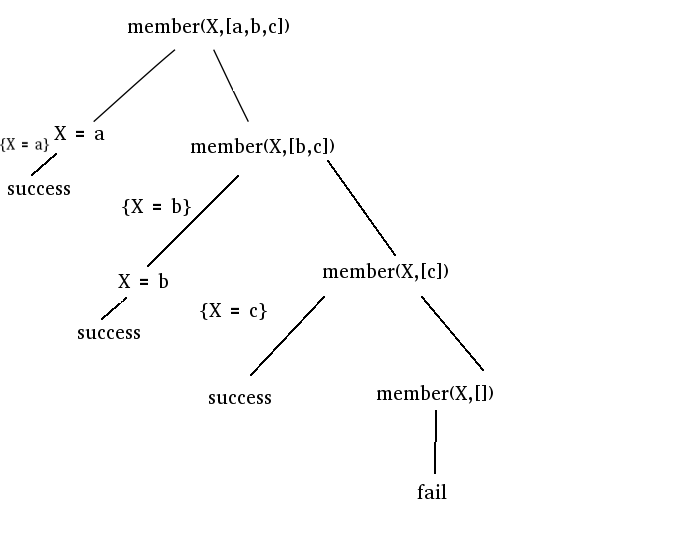
\includegraphics[scale=0.45]{resolution_2.png}
\end{center}	

\end{frame}

\begin{frame}{Training time !}

	Some exercices are available in the documents at your disposal.\\ Go through them and good luck :)

\end{frame}


\end{document}
